% Options for packages loaded elsewhere
\PassOptionsToPackage{unicode}{hyperref}
\PassOptionsToPackage{hyphens}{url}
%
\documentclass[
  man]{apa6}
\usepackage{amsmath,amssymb}
\usepackage{lmodern}
\usepackage{iftex}
\ifPDFTeX
  \usepackage[T1]{fontenc}
  \usepackage[utf8]{inputenc}
  \usepackage{textcomp} % provide euro and other symbols
\else % if luatex or xetex
  \usepackage{unicode-math}
  \defaultfontfeatures{Scale=MatchLowercase}
  \defaultfontfeatures[\rmfamily]{Ligatures=TeX,Scale=1}
\fi
% Use upquote if available, for straight quotes in verbatim environments
\IfFileExists{upquote.sty}{\usepackage{upquote}}{}
\IfFileExists{microtype.sty}{% use microtype if available
  \usepackage[]{microtype}
  \UseMicrotypeSet[protrusion]{basicmath} % disable protrusion for tt fonts
}{}
\makeatletter
\@ifundefined{KOMAClassName}{% if non-KOMA class
  \IfFileExists{parskip.sty}{%
    \usepackage{parskip}
  }{% else
    \setlength{\parindent}{0pt}
    \setlength{\parskip}{6pt plus 2pt minus 1pt}}
}{% if KOMA class
  \KOMAoptions{parskip=half}}
\makeatother
\usepackage{xcolor}
\usepackage{graphicx}
\makeatletter
\def\maxwidth{\ifdim\Gin@nat@width>\linewidth\linewidth\else\Gin@nat@width\fi}
\def\maxheight{\ifdim\Gin@nat@height>\textheight\textheight\else\Gin@nat@height\fi}
\makeatother
% Scale images if necessary, so that they will not overflow the page
% margins by default, and it is still possible to overwrite the defaults
% using explicit options in \includegraphics[width, height, ...]{}
\setkeys{Gin}{width=\maxwidth,height=\maxheight,keepaspectratio}
% Set default figure placement to htbp
\makeatletter
\def\fps@figure{htbp}
\makeatother
\setlength{\emergencystretch}{3em} % prevent overfull lines
\providecommand{\tightlist}{%
  \setlength{\itemsep}{0pt}\setlength{\parskip}{0pt}}
\setcounter{secnumdepth}{-\maxdimen} % remove section numbering
% Make \paragraph and \subparagraph free-standing
\ifx\paragraph\undefined\else
  \let\oldparagraph\paragraph
  \renewcommand{\paragraph}[1]{\oldparagraph{#1}\mbox{}}
\fi
\ifx\subparagraph\undefined\else
  \let\oldsubparagraph\subparagraph
  \renewcommand{\subparagraph}[1]{\oldsubparagraph{#1}\mbox{}}
\fi
\newlength{\cslhangindent}
\setlength{\cslhangindent}{1.5em}
\newlength{\csllabelwidth}
\setlength{\csllabelwidth}{3em}
\newlength{\cslentryspacingunit} % times entry-spacing
\setlength{\cslentryspacingunit}{\parskip}
\newenvironment{CSLReferences}[2] % #1 hanging-ident, #2 entry spacing
 {% don't indent paragraphs
  \setlength{\parindent}{0pt}
  % turn on hanging indent if param 1 is 1
  \ifodd #1
  \let\oldpar\par
  \def\par{\hangindent=\cslhangindent\oldpar}
  \fi
  % set entry spacing
  \setlength{\parskip}{#2\cslentryspacingunit}
 }%
 {}
\usepackage{calc}
\newcommand{\CSLBlock}[1]{#1\hfill\break}
\newcommand{\CSLLeftMargin}[1]{\parbox[t]{\csllabelwidth}{#1}}
\newcommand{\CSLRightInline}[1]{\parbox[t]{\linewidth - \csllabelwidth}{#1}\break}
\newcommand{\CSLIndent}[1]{\hspace{\cslhangindent}#1}
\ifLuaTeX
\usepackage[bidi=basic]{babel}
\else
\usepackage[bidi=default]{babel}
\fi
\babelprovide[main,import]{english}
% get rid of language-specific shorthands (see #6817):
\let\LanguageShortHands\languageshorthands
\def\languageshorthands#1{}
% Manuscript styling
\usepackage{upgreek}
\captionsetup{font=singlespacing,justification=justified}

% Table formatting
\usepackage{longtable}
\usepackage{lscape}
% \usepackage[counterclockwise]{rotating}   % Landscape page setup for large tables
\usepackage{multirow}		% Table styling
\usepackage{tabularx}		% Control Column width
\usepackage[flushleft]{threeparttable}	% Allows for three part tables with a specified notes section
\usepackage{threeparttablex}            % Lets threeparttable work with longtable

% Create new environments so endfloat can handle them
% \newenvironment{ltable}
%   {\begin{landscape}\centering\begin{threeparttable}}
%   {\end{threeparttable}\end{landscape}}
\newenvironment{lltable}{\begin{landscape}\centering\begin{ThreePartTable}}{\end{ThreePartTable}\end{landscape}}

% Enables adjusting longtable caption width to table width
% Solution found at http://golatex.de/longtable-mit-caption-so-breit-wie-die-tabelle-t15767.html
\makeatletter
\newcommand\LastLTentrywidth{1em}
\newlength\longtablewidth
\setlength{\longtablewidth}{1in}
\newcommand{\getlongtablewidth}{\begingroup \ifcsname LT@\roman{LT@tables}\endcsname \global\longtablewidth=0pt \renewcommand{\LT@entry}[2]{\global\advance\longtablewidth by ##2\relax\gdef\LastLTentrywidth{##2}}\@nameuse{LT@\roman{LT@tables}} \fi \endgroup}

% \setlength{\parindent}{0.5in}
% \setlength{\parskip}{0pt plus 0pt minus 0pt}

% Overwrite redefinition of paragraph and subparagraph by the default LaTeX template
% See https://github.com/crsh/papaja/issues/292
\makeatletter
\renewcommand{\paragraph}{\@startsection{paragraph}{4}{\parindent}%
  {0\baselineskip \@plus 0.2ex \@minus 0.2ex}%
  {-1em}%
  {\normalfont\normalsize\bfseries\itshape\typesectitle}}

\renewcommand{\subparagraph}[1]{\@startsection{subparagraph}{5}{1em}%
  {0\baselineskip \@plus 0.2ex \@minus 0.2ex}%
  {-\z@\relax}%
  {\normalfont\normalsize\itshape\hspace{\parindent}{#1}\textit{\addperi}}{\relax}}
\makeatother

\makeatletter
\usepackage{etoolbox}
\patchcmd{\maketitle}
  {\section{\normalfont\normalsize\abstractname}}
  {\section*{\normalfont\normalsize\abstractname}}
  {}{\typeout{Failed to patch abstract.}}
\patchcmd{\maketitle}
  {\section{\protect\normalfont{\@title}}}
  {\section*{\protect\normalfont{\@title}}}
  {}{\typeout{Failed to patch title.}}
\makeatother

\usepackage{xpatch}
\makeatletter
\xapptocmd\appendix
  {\xapptocmd\section
    {\addcontentsline{toc}{section}{\appendixname\ifoneappendix\else~\theappendix\fi\\: #1}}
    {}{\InnerPatchFailed}%
  }
{}{\PatchFailed}
\keywords{habit, sequence, routine, dopamine, mindfulness, visual search, eye-movements\newline\indent Word count: 8274}
\DeclareDelayedFloatFlavor{ThreePartTable}{table}
\DeclareDelayedFloatFlavor{lltable}{table}
\DeclareDelayedFloatFlavor*{longtable}{table}
\makeatletter
\renewcommand{\efloat@iwrite}[1]{\immediate\expandafter\protected@write\csname efloat@post#1\endcsname{}}
\makeatother
\usepackage{lineno}

\linenumbers
\usepackage{csquotes}
\ifLuaTeX
  \usepackage{selnolig}  % disable illegal ligatures
\fi
\IfFileExists{bookmark.sty}{\usepackage{bookmark}}{\usepackage{hyperref}}
\IfFileExists{xurl.sty}{\usepackage{xurl}}{} % add URL line breaks if available
\urlstyle{same} % disable monospaced font for URLs
\hypersetup{
  pdftitle={Assessing the influence of dopamine and mindfulness on the formation of routines in visual search},
  pdfauthor={*Kelly G. Garner1,2, Li-Ann Leow2, Aya Uchida2, Christopher Nolan1, Ole Jensen3, Marta I. Garrido4, \& Paul E. Dux2},
  pdflang={en-EN},
  pdfkeywords={habit, sequence, routine, dopamine, mindfulness, visual search, eye-movements},
  hidelinks,
  pdfcreator={LaTeX via pandoc}}

\title{Assessing the influence of dopamine and mindfulness on the formation of routines in visual search}
\author{*Kelly G. Garner\textsuperscript{1,2}, Li-Ann Leow\textsuperscript{2}, Aya Uchida\textsuperscript{2}, Christopher Nolan\textsuperscript{1}, Ole Jensen\textsuperscript{3}, Marta I. Garrido\textsuperscript{4}, \& Paul E. Dux\textsuperscript{2}}
\date{}


\shorttitle{Dopamine, mindfulness and visual search}

\authornote{

*denotes corresponding author: \href{mailto:kelly.grace.garner@unsw.edu.au}{\nolinkurl{kelly.grace.garner@unsw.edu.au}}

This project has received funding from the European Union's Horizon 2020 research and innovation programme under the Marie Sklodowska-Curie grant agreement No 796329, awarded to Kelly Garner. MIG was supported by the Centre of Excellence for Integrative Brain Function (CE140100007). PED was supported by a grant from the Australian Research Council (DP210101977). We thank Prof.~Fred Westbrook for feedback on an earlier draft and insightful discussions about this work.

The data is available at UQ eSpace. Task code and analysis code are available on github. {[}Note: links will be made available once a version of this manuscript has been accepted for publication{]}.

Correspondence concerning this article should be addressed to *Kelly G. Garner. E-mail: \href{mailto:kelly.grace.garner@unsw.edu.au}{\nolinkurl{kelly.grace.garner@unsw.edu.au}}

}

\affiliation{\vspace{0.5cm}\textsuperscript{1} School of Psychology, University of New South Wales, Australia\\\textsuperscript{2} School of Psychology, University of Queensland, Australia\\\textsuperscript{3} School of Psychology, University of Birmingham, UK\\\textsuperscript{4} Melbourne School of Psychological Sciences and Graeme Clark Institute for Biomedical Engineering, University of Melbourne, Australia}

\begin{document}
\maketitle

Data: \href{https://doi.org/10.48610/a6a65c7}{10.48610/a6a65c7}\\
Task code: \href{https://zenodo.org/doi/10.5281/zenodo.10637596}{10.5281/zenodo.10637597}\\
Analysis code: \href{https://zenodo.org/doi/10.5281/zenodo.10637592}{10.5281/zenodo.10637593}

\clearpage

\hypertarget{abstract}{%
\section{Abstract}\label{abstract}}

Given experience in cluttered but stable visual environments, our eye-movements form stereotyped routines that sample task-relevant locations, while not mixing-up routines between similar task-settings. Both dopamine signalling and mindfulness have been posited as factors that influence the formation of such routines, yet quantification of their impact remains to be tested in healthy humans. Over two sessions, participants searched through grids of doors to find hidden targets, using a gaze-contingent display. Within each session, door scenes appeared in either one of two colours, with each colour signalling a differing set of likely target locations. We derived measures for how well target locations were learned (target-accuracy), how routine were sets of eye-movements (stereotypy), and the extent of interference between the two scenes (setting-accuracy). Participants completed two sessions, where they were administered either levodopa (dopamine precursor) or placebo (vitamin C), under double-blind counterbalanced conditions. Dopamine and trait mindfulness (assessed by questionnaire) interacted to influence both target-accuracy and stereotypy. Increasing dopamine improved accuracy and reduced stereotypy for high mindfulness scorers, but induced the opposite pattern for low mindfulness scorers. Dopamine also disrupted setting-accuracy invariant to mindfulness. Our findings show that mindfulness modulates the impact of dopamine on the target-accuracy and stereotypy of eye-movement routines, whereas increasing dopamine promotes interference between task-settings, regardless of mindfulness. These findings provide a link between non-human and human models regarding the influence of dopamine on the formation of task-relevant eye-movement routines, and provide novel insights into behaviour-trait factors that modulate the use of experience when building adaptive repertoires.

\clearpage

\hypertarget{introduction}{%
\section{Introduction}\label{introduction}}

\label{sec:Introduction}

Given stable environmental contingencies, it is adaptive for an organism to develop routine ways of performing tasks requiring multiple responses. Dopamine is assumed to play a key role in the neural computations that underlie the formation of task routines. A large body of evidence shows that dopaminergic midbrain neurons encode reward prediction errors between stimulus-outcome associations (Hollerman \& Schultz, 1998; e.g. Schultz, Apicella, \& Ljungberg, 1993; Waelti, Dickinson, \& Schultz, 2001), and such errors are assumed to underpin the teaching signal that computes the value of actions (Sutton \& Barto, 2018). A comparable signal generated in striatum marks the difference between expected and actual saccadic sequence lengths used by macaques to attain reward during visual search (Desrochers, Amemori, \& Graybiel, 2015; Desrochers, Jin, Goodman, \& Graybiel, 2010). This signal is assumed to reflect a cost-benefit signal that computes the value of saccadic routines. There also exists a large body of evidence from rodent and macaque models suggesting that increased striatal dopamine availability speeds the transition from goal-directed to habitual control of behaviour (Harmer \& Phillips, 1998; Nadel et al., 2021, 2021; Nelson \& Killcross, 2006), the latter of which is assumed to underlie performance of routines (Desrochers et al., 2015; Dezfouli \& Balleine, 2012; Dezfouli, Lingawi, \& Balleine, 2014; Graybiel \& Grafton, 2015; Smith \& Graybiel, 2016). Although this evidence implicates dopamine in the formation of task-relevant routines, whether dopamine availability modulates the formation of saccadic routines in humans remains an open question.

One way to address this question is to increase dopamine availability via administration of levodopa, a precursor to dopamine. levodopa administration in humans has been associated with increased striatal activity in response to positive reward prediction errors, assessed using blood-oxygenation-level-dependent BOLD responses (Pessiglione, Seymour, Flandin, Dolan, \& Frith, 2006), and with reduction of exploratory choices during instrumental learning (Chakroun, Mathar, Wiehler, Ganzer, \& Peters, 2020; Shohamy, Myers, Geghman, Sage, \& Gluck, 2006). This suggests that levodopa may increase the perceived value of actions by inducing optimistic evaluations of outcomes (FitzGerald, Dolan, \& Friston, 2015), possibly by disrupting feedback processing (Shohamy et al., 2006). Elevating dopamine availability via levodopa may therefore have a comparable impact on the cost-benefit computations driving the formation of saccadic routines during visual search. Specifically, levodopa may promote an optimistic evaluation of the performed sequence, increasing the probability that it is adopted as a routine.

For task-oriented routines to be adaptive, it is also required that they are not mixed-up between tasks, despite overlap in the situational cues and actions that mark task environments. Here we define mix-ups as the performing behaviours that are relevant for the task that is not currently being performed, and we refer to this as task-interference. More broadly, dopamine is assumed to play a modulatory role in the activation of task-relevant behaviours in response to relevant situational cues (Budzillo, Duffy, Miller, Fairhall, \& Perkel, 2017), as well as promoting the formation of routines. Patients with Parkinson's Disease consistently show deficits switching between simple sensorimotor tasks (R. Cools, Barker, Sahakian, \& Robbins, 2001; Wiecki \& Frank, 2010), as do healthy participants who have been administered D2 antagonists (Mehta, Manes, Magnolfi, Sahakian, \& Robbins, 2004). Such findings have been accounted for by assuming that decreased dopamine causes increased uncertainty about the probability of being in a specific task-state (Friston et al., 2012). These assumptions are based on evidence from constrained tasks - i.e.~when single correct responses are required for given stimuli. In contrast, saccadic routines are often formed from a self-selected set of many possible eye-movements, and it is unclear whether dopamine modulates switching between such routines. If a modulation is observed, it is unclear whether the effect of increasing dopamine is opposite to that of depleted dopamine, i.e.~does increasing dopamine availability promote segregation of task routines? Or, does increasing dopamine availability make it more difficult to switch between routines, thereby increasing the probability of interference between them?

A further but less frequently discussed component of the processes underlying task routine learning and deployment, is the brain's execution of task-relevant cues and actions. Presumably, the organism that encodes an accurate representation of cues, actions and outcomes is at an adaptive advantage when forming and executing task-relevant routines. A growing body of empirical evidence suggests that mindfulness may modulate such representations. Mindfulness has been defined as a mental state that emphasises current sensory and internal inputs (Davids, 1900; Shapiro, Carlson, Astin, \& Freedman, 2006), and as such is well-placed to promote accurate task-representations. In support of this, mindfulness practice has been associated with increased error monitoring during cognitively challenging tasks (Andreu et al., 2017), and with greater sensitivity to dynamics in operant reinforcement contingencies (Chen \& Reed, 2023; Reed, 2023). This suggests that increased mindfulness is associated with better differentiation between current and previous contingencies of reinforcement, potentially via improved focus on the \textcolor{blue}{current contingencies}, thereby reducing interference \textcolor{blue}{from previous contingencies}. Mindfulness has been shown to vary at the trait level and is assessable using standardized questionnaires (e.g.~Baer et al, (2006)).

What could be the modulatory influence of mindfulness on the formation and deployment of task-relevant routines? The influence of mindfulness on routine learning and task-switching may be opposing to the influence of dopamine: individuals low in trait mindfulness are faster to exploit sequential regularities in stimulus-response tasks (Stillman, Feldman, Wambach, Howard, \& Howard, 2014), and exploitation of such regularities are assumed to support habitual responses (Dezfouli \& Balleine, 2012; Dezfouli et al., 2014). Mindfulness may also promote task-switching; higher levels of trait mindfulness have been associated with decreased reliance on past behaviours when stimuli are conserved across tasks that carry different cognitive demands (Greenberg, Reiner, \& Meiran, 2012; Kuo \& Yeh, 2015). Indeed, both the reinforcement learning (RL) and active inference frameworks have been used to posit that mindfulness and dopamine engage common mechanisms; increased mindfulness attenuates striatal reward prediction errors (Kirk \& Montague, 2015; Kirk, Pagnoni, Hétu, \& Montague, 2019), possibly via greater regulation from stronger cortical
representations of subjective values and internal states (Kirk, Gu, Harvey, Fonagy, \& Montague, 2014). In the active inference framework, both dopamine (FitzGerald et al., 2015; Friston et al., 2012) and mindfulness (Giommi et al., 2023; Laukkonen \& Slagter, 2021) are assumed to increase the salience of task relevant cues, by increasing certainty of the estimates of their value. Although increasing dopamine will increase the salience of any cue present, mindfulness prioritises the salience of goal-relevant cues. These theories therefore posit that mindfulness may buffer against the influence of elevated dopamine, either by attenuating elevated reward prediction errors, or by further amplifying the salience of cues according to their goal-relevance. Despite these assumed common mechanisms of influence, it remains to be quantitatively tested whether mindfulness interacts with dopamine during the performance and execution of task-relevant visual routines.

Using a novel protocol designed to test the formation and execution of task-relevant saccadic routines in humans, we sought to test whether administration of levodopa increased suboptimal routine formation, and whether increased dopamine modulated interference between routines. We further sought to test whether higher levels of trait mindfulness provided a buffer against the impacts of increased dopamine availability. To preview the results, levodopa decreased target-accuracy and promoted routine formation in individuals with low trait-mindfulness, whereas high trait-mindfulness was associated with the opposite pattern. Regardless of mindfulness, dopamine increased task-interference.

\hypertarget{methods}{%
\section{Methods}\label{methods}}

\label{sec:Methods}

All the data from this study is available at UQ eSpace\footnote{DOI: 10.48610/a6a65c7}. Task code\footnote{DOI: 10.5281/zenodo.10637597}, analysis code and code to produce the manuscript\footnote{DOI: 10.5281/zenodo.10637593} are available on github.

The experiment and analysis plan were \href{DOI:\%2010.17605/OSF.IO/XN6D2}{pre-registered} on the Open Science Framework\footnote{DOI: 10.17605/OSF.IO/XN6D2}.

\hypertarget{participants}{%
\subsection{Participants}\label{participants}}

\label{sec:Participants}

A total of 40 participants (mean age: 24.5, sd: 5, 30 female, 10 male) were recruited using the undergraduate and paid SONA pools administered by the University of Queensland. All procedures were cleared by the University of Queensland Human Research ethics committee {[}2017/HE000847{]}, and were conducted in accordance with the National Statement on Ethical Conduct in Human Research. Participants were over 18 years old, had no known neurological or psychiatric conditions (assessed by self report), and no contraindications to levodopa, as assessed by the levodopa safety screening questionnaire. Informed consent was obtained at the start of the first session.

\hypertarget{procedure}{%
\subsection{Procedure}\label{procedure}}

\label{sec:Procedure}

Participants attended two sessions, spaced approximately one week apart. After initial blood pressure (BP) and mood assessments (Bond \& Lader, 1974), participants received either placebo (vitamin C) or levodopa (Madopar 125: 100 mg levodopa and 25 mg Benserazide Hydrochloride), crushed and dispersed in orange juice, now referred to as the `placebo' and `dopamine' sessions respectively. The solution was prepared by an experimenter who did not administer the remaining experimental procedures. This protocol was sufficient to achieve double blinding in previous work (Chowdhury, Guitart-Masip, Bunzeck, Dolan, \& Düzel, 2012; Chowdhury et al., 2013). Participants then completed the Five Facet Mindfulness Questionnaire (Baer et al., 2006). \textcolor{blue}{This is a 15 item self-report questionnaire that measures mindfulness with regards to thoughts and experiences in daily life. It includes items such as 'I don't pay attention to what I'm doing because I'm daydreaming, worrying, or otherwise distracted' and 'I do jobs or tasks automatically without being aware of what I'm doing'. Participants also completed} the Barratt Impulsivity Scale {[}BIS; Patton, Stanford, and Barratt (1995){]}, as trait impulsivity scores are associated with midbrain dopamine D2/D3 receptor availability (Buckholtz et al., 2010). Around 30 minutes after drug administration, participants completed a second BP and mood rating assessment. Participants then completed the practice stage of the task, so that the experimental stage began approximately 40 minutes after drug ingestion, within the window of peak plasma availability (Contin \& Martinelli, 2010). At the end of the session, participants completed the final BP and mood rating assessment and were asked whether they thought they had been given the active or placebo drug.

\hypertarget{apparatus}{%
\subsection{Apparatus}\label{apparatus}}

\label{sec:Apparatus}

The experimental task was run with custom code, written using Matlab 2012b (32 bit) and Psychtoolbox v3.0.14, on a Windows 7 (64-bit) on a Dell Precision T1700 desktop computer, displayed using a ASUS VG248 monitor. Gaze coordinates (x, y) were sampled at 120 Hz using a monitor-mounted iView Red-m infrared eye tracker (SensoMotoric Instruments GmbH, Teltow, Germany). Participants were seated from the monitor at an approximate viewing distance of 57 cm, and positioned on a chin-rest for the duration of the task.

\hypertarget{experimental-task}{%
\subsection{Experimental Task}\label{experimental-task}}

\label{sec:Experimental Task}

Each trial began with a fixation dot presented centrally on a grey screen {[}RGB: 200 200 200{]}. Participants were instructed to fixate on the dot to begin a trial. After 1000 ms of continuous correct fixation samples (within 100 pixels of fixation), a square was presented that comprised 18° visual angle along each length. The square could be one of four possible colours {[}RGBs: 87, 208, 169; 267, 145, 52; 167, 162, 229; 239, 91, 158{]}. After 1000 ms, a 4 x 4 grid of smaller squares appeared within the larger square, in a darker version of the background colour ({[}RGB{]}-50). Each square comprised 2.6°. Participants were instructed that the 4 x 4 grid represented doors, and that they were to use their eyes to open the doors to find where the target was hiding. Participants were instructed that they were to fixate on a single door to open it (see Fig \ref{fig:taskfig}A). When participants had fixated on a door for over 300 ms, the door either turned black {[}RGB: 50, 50, 50{]}, to denote the absence of a target, or the target was displayed and the trial was terminated. If the door had turned black, it returned to its previous colour as soon as it was detected that the participant had moved their eyes from the door \textcolor{blue}{[see Supplemental Figure 1, for a visual depiction]}. Targets were animal images drawn randomly on each trial from a pool of 100 images taken from the internet\footnote{The folder of target images can be downloaded from \href{https://github.com/kel-github/variability-decision-making/blob/master/iforage_DA_task_code_redSMI/tgt0-100.zip}{here}}. The time at which the target was available to be found varied from trial to trial, with the onset being drawn from a uniform distribution between 500-2000 ms. Once the target was available and the correct door selected, the target was displayed for 750 ms. Upon termination of the trial, the grey screen and white fixation cross were presented.

In each session, participants saw the display in two possible colours. Participants were instructed that each colour represented a world, and that the animals had different places they preferred to hide, depending on the world they were in. There were four possible target locations within each world, or from here on, each setting. For each setting, one door from each quadrant was selected as one of the four possible target locations (see Fig \ref{fig:taskfig}B), with the constraint that target locations could not overlap between settings. Thus each colour reflected a setting in which participants could establish a set of task-relevant eye-movements, i.e.~towards the 4 possible target locations. Note that within each setting, the target was equally likely to appear behind any one of the 4 target doors (p=.25) and would never appear behind the remaining doors (p=0). Colour-target location mappings were counterbalanced across participants, as was the assignment of colours to sessions. Participants completed 80 trials in each setting. Eye-movement calibration and validation was performed every 20 trials. Participants were also shown the standard QWERTY keyboard and were instructed that they could press `x' at any time to perform a new calibration and validation if they felt that their eye-movements were no longer being registered accurately.

\begin{figure}

{\centering 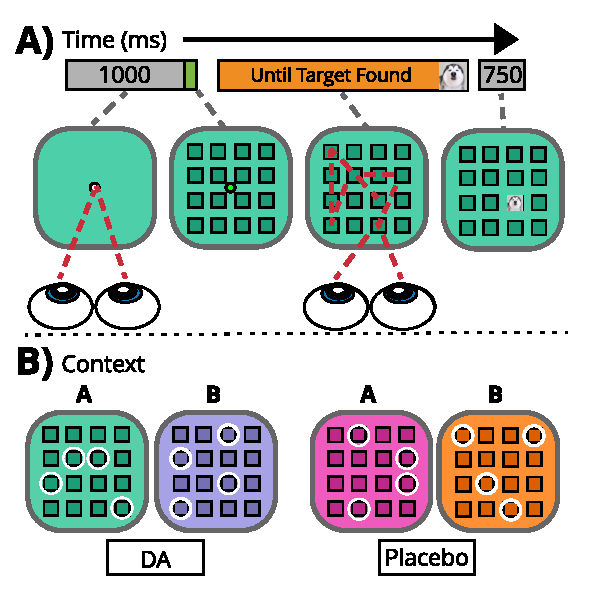
\includegraphics[width=0.7\linewidth]{../../images/DA_ExpTask_RR1} 

}

\caption{Experimental Task. A) A single trial where participants use their eyes to open doors to locate an animal image target. B) Contexts and sessions: in each session, participants are exposed to two colour contexts each with 4 unique and equiprobable target locations. Colours and target locations were counterbalanced across participants and sessions. In each session, levodopa (DA) or placebo is administered under double blind conditions.}\label{fig:taskfig}
\end{figure}

\hypertarget{statistical-approach}{%
\subsection{Statistical Approach}\label{statistical-approach}}

\label{sec:Statistical Approach}

The analysis was designed to assess how well participants learned the target locations, the extent to which participants formed a routine for door selections (how stereotypical they became in their order of door-selections), and how well they disambiguated between settings. We modelled how these elements of performance were modulated by the dopamine and mindfulness factors. All custom analysis code is available online. The analysis was performed using R and RStudio v2022.07.2 (RStudio Team, 2020), and can be reproduced in the Neurodesk container environment (Renton et al., 2022).

\hypertarget{data-cleaning}{%
\subsubsection{Data cleaning}\label{data-cleaning}}

\label{sec:Data cleaning}

We asserted that a door could not be selected twice consecutively, thus any consecutive selections were classified as a single selection. As the final door selection of every trial was fixed (i.e.~finding the target location ends the trial), we removed the final selection from each trial for the stereotypy (routine) analysis defined below. We excluded data from one participant whose total number of door selections was greater than 3 standard deviations from the mean across both sessions. The remaining 39 datasets were retained for all of the analyses. Note that this is more inclusive than our pre-registered plan for data exclusions\footnote{DOI: 10.17605/OSF.IO/XN6D2}. Based on pilot data, we had planned to exclude participants who scored \textless{} 65\% accuracy over the course of a session. Analysis of the final sample suggested that this was too stringent, as this resulted in the exclusion of 14 of 40 participants. We have not analysed the data with the exclusion of these participants, owing to the large drop in statistical power for the individual differences component of the analysis.

\hypertarget{target-accuracy}{%
\subsection{Target-Accuracy}\label{target-accuracy}}

\label{sec:Target-Accuracy}

We first sought to determine the extent to which levodopa and mindfulness influenced the learning of target locations (target-accuracy). Data was grouped into blocks of 10 trials per setting, and grouped across settings, resulting in 8 blocks of 20 trials. We computed for each block the proportion of door selections that were target relevant (TR) given the current setting (i.e.~the setting presented on trial t). We assessed the influence of block, drug and mindfulness on target-accuracy using Bayesian mixed-model logistic regression. Target-accuracy was assumed to be drawn from a binomial distribution (1=target door, 0=non-target door). We then estimated the probability of drawing a target-door from the total number of door selections, using a logit link function to convert probabilities to log-odds. Thus the resulting regression parameter values reflect changes to the log-odds of accurate door selections.

For this and following analyses, we identified the model that best fit the data, and made inference over the resulting parameters. We report the 95\% confidence intervals (CIs) of the parameter posteriors, and assume a reliable effect when the 95\% CIs do not include zero. Models were fit using the BRMS (Bürkner, 2017) interface for Stan (Team, n.d.) and RStan (Stan Development Team, 2023). We used the default weakly informative priors as specified in Burkner (2017). Specifically, fixed and random effect \(\beta\) coefficients were given a flat prior, intercept and standard deviations were assumed to be drawn from a student's \(t\) distribution (df=1, location=0, scale=2.5), and the LKJ-correlation prior with parameter \(\zeta\) \textgreater{} 0 was used for the parameter covariance matrix. For each model, we checked for parameter recovery using simulated data. Once fitted, we checked that the residuals showed no signs of systematic error, that the chains had converged, and that \(\hat{R}\) values were less than 1.01, as this suggests that the model has converged.

To eschew an overly large model space, and in line with our pre-registration, we first fit models that contained each possible combination of the block and drug regressors (and associated random effects), and found the best model using leave-one-out (LOO) cross validation, as implemented in Vehtari et al., (2017). Rather than re-fitting the model for every sub-sample, which is computationally expensive, this algorithm instead computes analytically how the predictions made by the model are influenced by each data point. The relationship between this influence and the change in the posterior that would occur as a consequence of holding out each data point can be used to compute the expected log-pointwise predictive density (ELPD). This quantifies the error that would occur in the prediction of each data point, when that data point is withheld from the model fitting procedure. The resulting ELPDs are then compared between models. We report the ELPD difference between the winning model and the next best models (a negative value indicates preference for the winning model). As the ELPD is computed using each observed data point, it is possible to estimate the standard error (SE) of the difference between models (Vehtari et al, (2017)). We therefore also report the ratio of the ELPD difference to the SE, as this provides a proxy for statistical significant differences between models. (Note that in the pre-registration document we had proposed to compare models using the deviance information criterion (DIC). As LOO is more robust than DIC to influential observations, and is readily implemented for use with BRMS model objects, we opted to use LOO instead of DIC).

Upon identifying the best model, we then added the mindfulness regressor, fitting all possible combinations, and once again selected the best model. Last we controlled for trait impulsivity by adding BIS scores as a main effect to the winning model. Note that in no cases did adding BIS scores improve the model. The full set of model comparisons are presented in the supplementary materials.

\hypertarget{setting-accuracy}{%
\subsection{Setting-Accuracy}\label{setting-accuracy}}

\label{sec:Setting-Accuracy}

We next sought to model the impact of levodopa and mindfulness on task interference. To measure the extent of task interference, we computed a measure of setting-accuracy. This measure indexes the total number of door selections (n) that were appropriate for the colour setting displayed on trial t (current setting, CS), relative to the number of door selections that were appropriate for the setting not displayed on trial t (i.e.~the other-setting from that session, OS):

\[
setting\mathrm{-}acc = \frac{\sum{CS_{n}}}{\sum{(CS_{n}, OS_{n})}}
\]

We modelled the influence of levodopa and mindfulness on setting-accuracy using the Bayesian mixed-effects logistic regression approach described above (Note that in the pre-registration document we had suggested to include a regressor for context. Visual inspection of the data showed that setting-accuracy was highly comparable across contexts {[}see Supplemental Figure 3{]}. We therefore opted to simplify the model space and collapse over this factor).

\hypertarget{stereotypical-door-selections}{%
\subsection{Stereotypical door selections}\label{stereotypical-door-selections}}

\label{sec:Stereotypical door selections}

Next, we determined the extent to which door-selections became routine over the course of the task - specifically, how much the order of door selections increased in stereotypy, and whether dopamine and mindfulness modulates the extent of stereotypy. Here we use stereotypy as a proxy for routine formation, and we define stereotypy as the tendency to choose doors in the same order, over trials (e.g. Desrochers et al., 2015).

In order to index stereotypy, we reasoned that stereotypy should result in an increase in the probability of a subset of door transitions. This stands in contrast to when making door selections in an exploratory, or non-stereotyped way, where there should be an even representation of door transition probabilities. Therefore, the transition probability matrices of individuals engaged in more stereotypical door selections should show higher variance than those who are not engaging in stereotypical door selections. We computed trial level transition probability matrices, and calculated the variance of each matrix. Variances were then collapsed across settings and trials to form a stereotypy score for each participant, session and block.\footnote{Note that we opted to index stereotypy using variance over transition probabilities as this measure captures consistent behaviours without over-penalizing slight variations between sequences. For example, the sequences x={[}1,2,3,4,5{]}, and y={[}1,2,4,3,5{]} share commonalities that are captured in a transition probability matrix that would not be captured by linear measures, such as comparing triplets between trials.}

The resulting stereotypy scores were subject to a comparable Bayesian mixture modelling approach as described above with a few key differences; the stereotypy scores were assumed to be drawn from a skewed normal distribution \(\mathcal{N}(\mu, \sigma, \alpha)\) whose mean (\(\mu\)) was defined by the regression parameters (the distribution of stereotypy scores are presented in Supplemental Figure 4). \(\sigma\) was assumed to be drawn from a Student's t distribution (df=3, location=0, scale=2.5), the skew parameter (\(\alpha\)) was assumed to be drawn from a normal distribution \(\mathcal{N}(0,4)\). The remaining priors for the intercept, beta-coefficients and parameter covariance matrix were defined in the same manner as for the accuracy data models. As the log-log plot of variances vs block suggested a power function, analysis was performed on the logged data. This ensured that the relationship between block and variance values was best described by a straight line. Identification of the winning model proceeded as described for the accuracy data above.

\hypertarget{blinding-analyses}{%
\subsection{Blinding analyses}\label{blinding-analyses}}

\label{sec:Blinding analyses}

To determine whether awareness of the dopamine intervention could have contributed to the findings, the probability of participant ratings were compared to the expected values assuming chance guessing, using a Chi Square test. BP and mood ratings were each subject to a session (dopamine vs placebo) x timepoint (pre-drug, pre-experiment, post-experiment) Bayesian repeated measures ANOVA, implemented using the BayesFactor package for R (Morey et al., 2023) using the default priors (Rouder, Morey, Speckman, \& Province, 2012).

\hypertarget{results}{%
\section{Results}\label{results}}

\label{sec:Results}

We investigated the impact of levodopa administration and trait mindfulness on the learning of task-relevant behaviour sets, and on the routine nature of their deployment. Participants opened doors to search for targets in a gaze-contingent display. The colour of the display signalled likely target locations, making some locations relevant for only that colour. We assessed how well participants learned target locations (target-accuracy), how routine was the order of door selections
across trials (stereotypy), and how well participants learned to segregate task-routines (setting-accuracy). Overall, mindfulness and dopamine interacted to influence the measures of target-accuracy and stereotypy; dopamine increased target-accuracy and reduced stereotypy for high mindfulness scorers, whereas dopamine decreased target-accuracy and increased stereotypy for low mindfulness scorers. Dopamine decreased setting-accuracy independent to mindfulness scores.

\hypertarget{target-accuracy-1}{%
\subsection{Target-Accuracy}\label{target-accuracy-1}}

\label{sec:Target-Accuracy Results}

\hypertarget{model-selection}{%
\subsubsection{Model selection}\label{model-selection}}

First we sought the best model in order to make subsequent inference over the parameters. In the first stage of model selection, the experimental factors of block (10 successive trials from each context, averaged across contexts), and drug (dopamine vs placebo) were used in a logistic regression to model the probability of a target door selection. We sought the combination of fixed and random effect factors that best accounted for the data. The winning model contained fixed main effects of block and drug. Although this model was only closely preferred to the next most complex model that contained a block x drug interaction (ELPD diff = -0.33, ELPD:SE = -0.57), it was strongly preferred to all other models (min ELPD diff = -958.53, ELPD:SE = -8.65).

We next sought to determine whether adding mindfulness scores improved the predictive accuracy of the model; the winning model contained an additional main effect of mindfulness, as well as block x mindfulness and drug x mindfulness interactions (ELPD diff to best model without mindfulness = -3.12, ELPD:SE = -0.62). Therefore the winning model to account for the data was:

\(\mathrm{\hat{y}} = \mathrm{block} + \mathrm{drug} + \mathrm{mind} + \mathrm{block*mind} + \mathrm{drug*mind} + \mathrm{(block:drug|sub)}\)

Adding BIS scores did not improve the predictive value of the model (ELPD diff = -1.95, ELPD:SE = -3.77). Note that although we draw inferences over parameters from the winning model, our inferences are the same as if we had used the more complex model that includes the BIS scores.

\hypertarget{the-effect-of-dopamine-and-mindfulness-on-target-accuracy}{%
\subsubsection{The effect of dopamine and mindfulness on target-accuracy}\label{the-effect-of-dopamine-and-mindfulness-on-target-accuracy}}

Having established the best model to account for the data, we next determined the influence of dopamine and mindfulness on target-accuracy by making inference over the resulting parameters. Target-accuracy data plotted by block x drug (dopamine vs placebo) are shown in Fig \ref{fig:accfig}A. Target-accuracy improved over blocks, and there was a small main effect of drug. These effects are described further below. However, critically, mindfulness and dopamine interacted to influence target-accuracy. The drug x mindfulness parameter differed reliably from zero (mean log odds = -0.08, 95\% CI{[}-0.12, -0.03{]}, see Fig \ref{fig:accfig}E).

To investigate this interaction, we computed mean target-accuracy change due to the drug session (\(\mu\) acc{[}dopamine - placebo{]}) for each participant. Note that a positive score indicates that performance was better in the dopamine session relative to placebo. Next we examined the relationship between dopamine-induced target-accuracy changes and mindfulness scores. As can be seen in Fig \ref{fig:accfig}B, there was a positive relationship between mindfulness and the influence of drug on target-accuracy. As mindfulness increased, so too did target-accuracy for the dopamine relative to the placebo session. For a numeric example, those scoring in the highest quartile showed mean target-accuracy scores of 0.47 (95\%CI{[}0.44, 0.50{]}) during the dopamine session, relative to mean target-accuracy scores of 0.41 (95\% CI{[}0.38, 0.43{]}) during the placebo session. Individuals scoring low on mindfulness numerically showed the opposite pattern (dopamine mean target-accuracy = 0.43, 95\% CI{[}0.41, 0.45{]}, placebo mean target-accuracy = 0.44, 95\%CI{[}0.43, 0.46{]}), note that Fig \ref{fig:accfig}B shows the difference between these scores). Thus the impact of dopamine on the establishment of task-relevant eye-movements is dependent on the mindfulness state of the individual.

Participants learned the target door locations over the course of the sessions, target-accuracy reliably increased over blocks. Mean target-accuracy in block 1 was 0.34 (95\% CI{[}0.32, 0.37{]}), relative to a block 8 mean of 0.51 (95\% CI{[}0.48, 0.53{]}). The model showed that the log-odds of a target door selection increased over blocks by an average of = 0.15, (95\% CI{[}0.08, 0.22, Fig \ref{fig:accfig}C, note that the model parameters are defined in log-odds because we used logistic regression). There was also the suggestion of a main effect of dopamine (mean log odds = 0.08, 95\% CI{[}0.035, 0.13, Fig \ref{fig:accfig}D), however, the impact of dopamine on target-accuracy is better explained by the drug x mindfulness interaction Fig \ref{fig:accfig}E). \textcolor{blue}{Although the winning model contained a block x mindfulness interaction, the 95\% CIs included zero} (mean log odds = 0.05, 95\% CI{[}-0.016, 0.12{]}, \textcolor{blue}{so we do not consider this parameter any further.}

\begin{figure}

{\centering 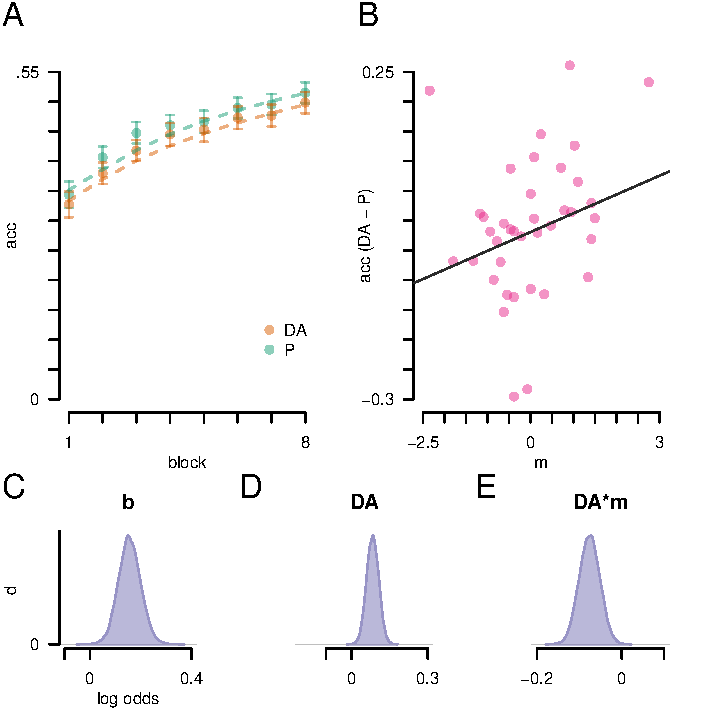
\includegraphics[width=0.7\linewidth]{../../images/acc_fig} 

}

\caption{The influence of dopamine and mindfulness on target-accuracy. A) Target-accuracy (t-acc) data by block and drug. Circles reflect observed average target-accuracy, dotted lines reflect the fit of the winning model. B) The association between trait mindfulness (x-axis) and the impact of drug on accuracy [dopamine-placebo]. The bottom row shows posterior densities (in log odds) estimated for C) the main effect of block (b), D) the main effect of dopamine, and E) the drug x mindfulness (m) interaction. DA = dopamine, P = placebo, d = density. Error bars reflect within-subject standard error of the mean [SE].}\label{fig:accfig}
\end{figure}

\hypertarget{setting-accuracy-1}{%
\subsection{Setting-Accuracy}\label{setting-accuracy-1}}

\label{sec:Setting-Accuracy Results}

\hypertarget{model-selection-1}{%
\subsubsection{Model selection}\label{model-selection-1}}

We first identified the model that best accounted for the influence of the experimental conditions on setting-accuracy. Comparable to the target-accuracy data, the best model contained fixed effects of block and drug, with no interactions. Although this model was only closely preferred to the next most complex model that contained a block x drug interaction (ELPD diff = -0.66, ELPD:SE = -1.67), it was strongly preferred to all other models (min ELPD diff = -553.79, ELPD:SE = -8.35).

Adding mindfulness scores improved the predictive accuracy of the model; the winning model contained an additional main effect of mindfulness (ELPD diff = -0.13, ELPD:SE = -0.12). Thus the winning model was:

\(\mathrm{\hat{y}} = \mathrm{block} + \mathrm{drug} + \mathrm{mind} + \mathrm{(block:drug|sub)}\)

Adding BIS scores did not improve the predictive value of the model (ELPD diff = -0.02, ELPD:SE = -0.03). Note that although we draw inferences over parameters from the winning model, our inferences are the same as if we had used the more complex model that includes the BIS scores.

\hypertarget{drug-and-not-mindfulness-impacts-setting-accuracy}{%
\subsubsection{Drug, and not mindfulness, impacts setting-accuracy}\label{drug-and-not-mindfulness-impacts-setting-accuracy}}

We next determined the influence of dopamine and mindfulness on setting-accuracy by making inference over the resulting model parameters. Dopamine reduced setting-accuracy; setting-accuracy was on average 0.64 (95\% CI {[}0.63, 0.65{]}) for the dopamine session, and 0.66 (95\% CI {[}0.65, 0.68{]}) for the placebo session (see Fig \ref{fig:caccfig}A). The log-odds of selecting a setting-accurate target door increased by a mean of 0.07 (95\% CI{[}0.01, 0.13, Fig \ref{fig:caccfig}B) for the placebo session, relative to the dopamine session. This suggests that dopamine caused interference between settings.

Setting-accuracy improved over blocks; mean accuracy in block 1 was 0.59 (95\% CI{[}0.58, 0.61{]}), relative to block 8 (mean: 0.69, 95\% CI{[}0.67, 0.71{]}). The model showed that the probability of selecting a setting relevant target door increased by a mean log odds of 0.13 (95\% CI{[}0.07, 0.19) per block (Fig \ref{fig:caccfig}C). In contrast to the target-accuracy data, the main effect of mindfulness was not a sufficiently reliable predictor of setting-accuracy (mean log odds = 0.04, 95\% CI{[}-0.04, 0.18{]}).

\begin{figure}

{\centering 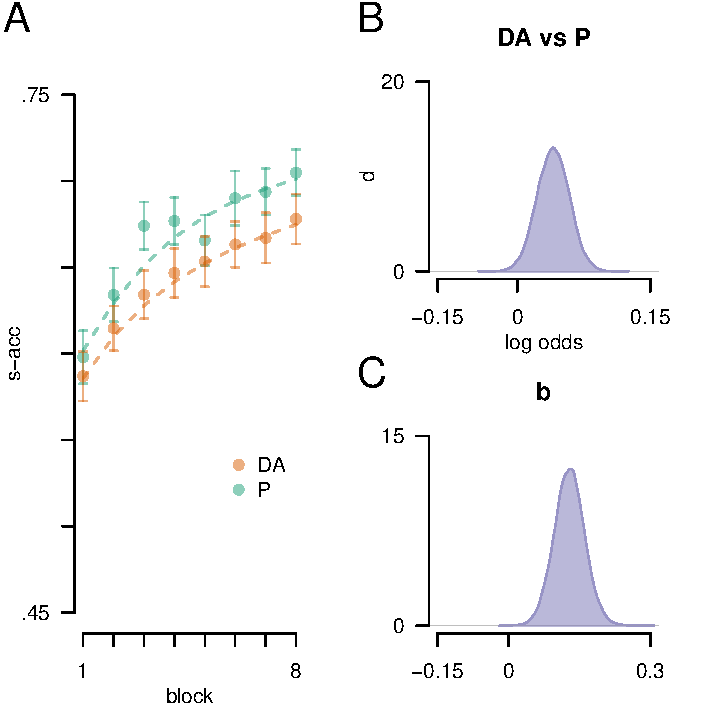
\includegraphics[width=0.7\linewidth]{../../images/cacc_fig} 

}

\caption{The influence of dopamine and mindfulness on setting-accuracy. A) Setting-Accuracy (s-acc) data by block and drug. Circles reflect observed average setting accuracy, dotted lines show the fit of the winning model. B) Estimated posterior density (in log odds) for the main effect of drug (dopamine vs placebo), D) same as in B, but for the main effect of block. DA = dopamine, P = placebo, b = block, d = density. Error bars reflect within-subject standard error of the mean [SE].}\label{fig:caccfig}
\end{figure}

\hypertarget{setting-accuracy-control-analysis}{%
\paragraph{Setting-accuracy control analysis}\label{setting-accuracy-control-analysis}}

Dopamine influences setting-accuracy, which indexes the likelihood of door selections that are relevant for the current-setting, relative to door selections that are relevant for the other-setting. As we exclude door selections for locations that are never target relevant from the computation of setting-accuracy, it is important to verify that setting-accuracy scores do indeed reflect interference between settings, rather than a general task learning deficit. To address this in an exploratory analysis, we reasoned that if setting-accuracy scores reflected a general deficit, then `error' door selections should be drawn randomly from not-target doors (other-setting = 4 \& neither = 8). A general deficit interpretation suggests that other-setting selections should be drawn from the total set (other-setting + neither) with \(p\) = \(\overline{.333}\). If setting-accuracy scores do reflect the presence of task-interference, then it would be likely that this error would be more common than a random door selection, therefore other-setting selections should occur at levels higher than chance. To test this, we computed for each participant the probability of other-setting selections, given the set of other-setting and neither door selections (\(p_{os}\)), and performed a one-sided t-test, against a null value of \(p\) = .333. (Note that we opted to use an NHST approach as we had a point null hypothesis). The \(p_{os}\) data was unlikely under the null hypothesis (mean = 0.37, 95\% CI{[}0.35, 0.39{]}, \(t\)(38) = 3.62, \(p\) = 0.0004. Therefore, we reject the hypothesis that the the dopamine induced drop in setting-accuracy reflects a general learning deficit.

\hypertarget{stereotypy-of-door-selections-routine}{%
\subsection{Stereotypy of door selections (routine)}\label{stereotypy-of-door-selections-routine}}

\label{sec:Stereotypy Results}

\hypertarget{model-selection-2}{%
\subsubsection{Model selection}\label{model-selection-2}}

We first sought the model that best explained the stereotypy data using the experimental predictors of block and drug. Note that we indexed stereotypy using the variance of transition probability matrices, where higher values indicates fewer likely transitions, and therefore higher stereotypy. The winning model contained main fixed effects of block and drug, and random effects for block x drug. Although this model was only closely preferred to the next most complex model that contained a block x drug interaction (ELPD diff = -0.26, ELPD:SE = -1.29), it was strongly preferred to all other models (min ELPD diff = -130.14, ELPD:SE = -7.71).

Adding mindfulness scores improved the ability of the model to account for the stereotypy data. The winning model contained an additional main effect of mindfulness and a drug x mindfulness interaction (ELPD diff = -3.15, ELPD:SE = -0.92). The winning model was:

\(\mathrm{\hat{y}} = \mathrm{block} + \mathrm{drug} + \mathrm{mind} + \mathrm{drug*mind} + \mathrm{(block:drug|sub)}\)

Adding BIS scores did not improve the predictive accuracy of the model (ELPD diff = -0.54, ELPD:SE = -1.41). Note that although we draw inferences over parameters from the winning model, our inferences are the same as if we had used the more complex model that includes the BIS scores.

\hypertarget{the-impact-of-drug-and-mindfulness-on-stereotypy}{%
\subsubsection{The impact of drug and mindfulness on stereotypy}\label{the-impact-of-drug-and-mindfulness-on-stereotypy}}

Stereotypy scores increased over blocks Fig \ref{fig:stereofig}A. Note that this increase is also in part due to increases in target-accuracy; as fewer doors are selected in error, the variance of the transition probability matrices increases. We first discuss the key results, and in the next section demonstrate their relationship to target-accuracy. Critically, mindfulness and dopamine interacted to impact stereotypy; we observed a reliable drug x mindfulness interaction (mean \(\beta\) = 0.11, 95\% CI{[}0.02, 0.21, Fig \ref{fig:stereofig}E). Mindfulness scores modulated the impact of dopamine on stereotypy. As a numerical example, those scoring in the highest quartile showed mean stereotypy scores of -8.74 (95\%CI{[}-8.80, -8.68{]}) during the dopamine session, relative to mean stereotypy scores of -8.68 (95\% CI{[}-8.74, -8.62{]}) during the placebo session. Individuals scoring low on mindfulness (lowest quartile) showed the opposite pattern (dopamine mean stereotypy = -8.69, 95\% CI{[}-8.75, -8.63{]}, placebo mean stereotypy = -8.72, 95\%CI{[}-8.78, -8.66{]}).

To visualise this interaction, we computed a mean variance change score between drug sessions for each participant (\(\mu\) stereotypy{[}dopamine - placebo{]}). Note that a positive score indicates that performance was more stereotyped in the dopamine session relative to placebo. As can be seen in Fig \ref{fig:stereofig}B, there was a negative relationship between drug-induced stereotypy changes and mindfulness. Specifically, higher mindfulness scorers showed lower stereotypy in the dopamine session compared to the placebo session. Low mindfulness scorers showed higher sterotypy in the dopamine session compared to the placebo session. Thus the impact of dopamine on the formation of eye-movement routines is dependent on the mindfulness state of the individual.

Participants developed more stereotypical routines over the course of the experiment, there was a clear main effect of block (mean increase per block: \(\beta\) = 0.32, 95\% CI{[}0.20, 0.43, Fig \ref{fig:stereofig}C). In line with the interaction of drug x mindfulness reported above, the main effect of mindfulness suggested a negative relationship with stereotypy (mindfulness mean \(\beta\) = -0.15, 95\% CI{[}-0.26, -0.05, Fig \ref{fig:stereofig}D). Overall, higher mindfulness scores predicted less stereotypy in door-selection patterns relative to low mindfulness scores.

\begin{figure}

{\centering 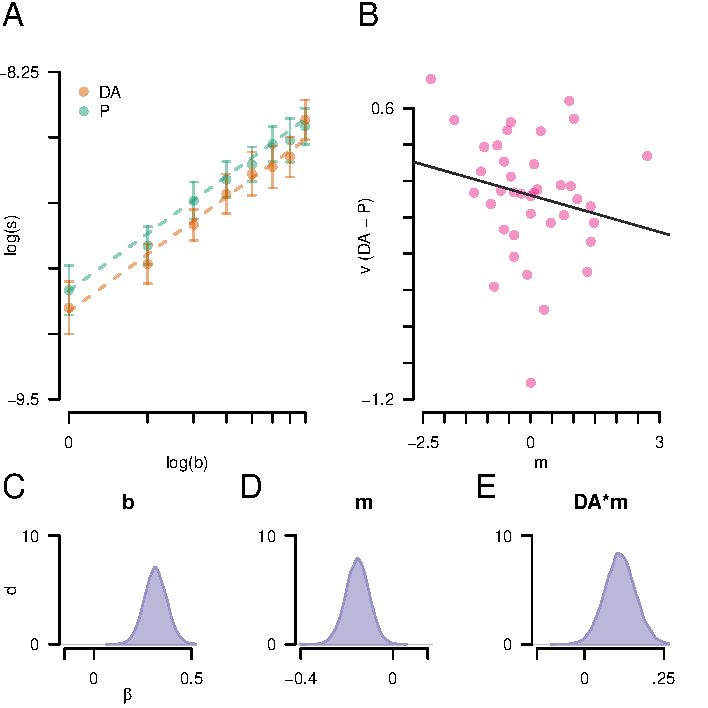
\includegraphics[width=0.7\linewidth]{../../images/s_fig} 

}

\caption{The influence of dopamine and mindfulness on door selection stereotypy. A) Log stereotypy scores by log block and drug. Circles reflect observed average variance (of the transition matrices), dotted lines show the fit of the winning model. B) The association between trait mindfulness (x-axis) and the impact of drug on variance [DA-P]. The bottom row shows posterior densities (in log odds) estimated for C) the main effect of block (b), D) the main effect of dopamine, and E) the drug x mindfulness (m) interaction. log(s) = log stereotypy scores, log(b) = block, DA = dopamine, P = placebo, b = block, m = mindfulness, DA*m = drug x mindfulness interaction, d = density. Error bars reflect within-subject standard error of the mean [SE].}\label{fig:stereofig}
\end{figure}

\hypertarget{on-the-relationship-between-target-accuracy-and-stereotypy}{%
\paragraph{On the relationship between target-accuracy and stereotypy}\label{on-the-relationship-between-target-accuracy-and-stereotypy}}

Accuracy and stereotypy showed opposing relationships with mindfulness and dopamine. Higher mindfulness scores were associated with dopamine-induced target-accuracy increases, and stereotypy decreases, relative to placebo. Individuals scoring low on mindfulness showed a deleterious influence of dopamine on target-accuracy, coupled with increased stereotypy, relative to placebo. As target-accuracy and stereotypy are possibly, but not necessarily related, we next sought to ensure that the observed influences of dopamine and mindfulness on stereotypy was not driven \textcolor{blue}{solely driven by its correlation with target-accuracy}, using an exploratory analyses. We reasoned that such a pattern of results could be observed if the measures of target-accuracy and stereotypy reflected a direct trade off; i.e.~as target-accuracy goes up, stereotypy goes down. A correlation analysis ruled out this possibility. We computed mean target-accuracy and stereotypy scores for each participant, collapsing across all experimental factors, and found that target-accuracy and stereotypy were positively related (\(r\)(37) = 0.81, \(p\) = 3.51e-10).

Next, to rule out the contribution of target-accuracy to the stereotypy results, we added mean target-accuracy, computed for each block and drug condition, as a regressor to the winning model. Adding target-accuracy as a regressor both clearly improved the predictive accuracy of the model (ELPD diff = -110.26, ELPD:SE = -6.12), and served to increase certainty in the interactive influence of mindfulness and drug on stereotypy scores. Specifically, the estimated influence of the interaction increased from \(\beta\) = 0.11 to \(\beta\) = 0.22 (95\% CI{[}0.14, 0.29{]}). Note that the pattern of remaining results were also consistent between the two models. Therefore, the data support the notion that mindfulness and dopamine interact to differently influence target-accuracy and stereotypy when participants perform task-relevant saccadic routines. Indeed, this data suggest that mindfulness and dopamine interacted to produce more erroneous routines. To visualise this, Fig \ref{fig:trajecfig} shows example door selections from two participants, one randomly selected from the lowest quartile of mindfulness scorers (top row), and one selected from the highest quartile of mindfulness scorers (bottom row). As can be seen, the low mindfulness scorer had adopted a routine that resulted in more erroneous door selections than the high mindfulness scorer. The low mindfulness scorer appears to have developed a suboptimal task strategy of trying all doors, regardless of task context.

\begin{figure}

{\centering 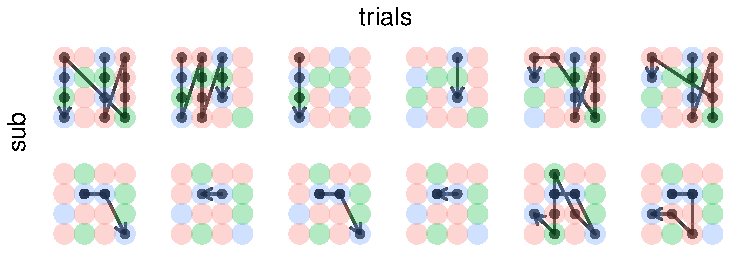
\includegraphics[width=0.7\linewidth]{../../images/trajectories2subs} 

}

\caption{Example door selection routines for two participants (rows) over 6 consecutive trials from the last block of the dopamine session. Door selections follow the order indicated by the arrow. Blue circles reflect target doors for that setting, and green doors are target doors for the other setting. Red doors are erroneous doors in that a target was never found there.}\label{fig:trajecfig}
\end{figure}

\hypertarget{blinding-check}{%
\subsection{Blinding check}\label{blinding-check}}

\label{sec:Blinding Results}

Next we checked if participants knew whether they had received levodopa or placebo across the two sessions. Participants were asked to report at the end of each session whether they thought they had received levodopa or placebo. Participant responses were coded as either correct for both sessions (cc: observed N = 7), correct for one session and incorrect for the other (ci: N = 11), or incorrect for both sessions (ii: N = 8). The probability of the observed guesses was not statistically unlikely given the null distribution of chance performance (the null hypothesis specified \(p\)= .25, .5, .25 for cc, ci, ii respectively, \(\chi^2\)(2, 26) = 0.69, \(p\) =0.71). Note that we were unable to include all the participants in this analysis owing to missing data. Specifically, due to a miscommunication in the research team, the blinding check questions contained `Don't know' as a possible response, for which we are unable to generate a null hypothesis. We therefore only include participants who made a guess using the levodopa and placebo options across both sessions.

\hypertarget{mood-and-blood-pressure}{%
\subsection{Mood and blood pressure}\label{mood-and-blood-pressure}}

We also sought to determine whether dopamine influenced physiological factors such as mood and blood pressure. For mood, the winning model contained a main effect of time-point and no other fixed effects. This model was preferred relative to next best model, which contained an additional main effect of drug (BF = 3.76, ±2.14\%) and was substantially preferred over the null random intercept model (BF = 514549 ±1.23\%).

Mean blood pressure was computed using the formula: Mean blood volume pulse (BVP) = diastolic blood pressure (DBP) + 1/3 {[}systolic blood pressure (SBP) -- DBP{]}. For mean BVP, the winning model contained main effects of both time-point and drug. This model was barely preferred to the next best model which contained a time-point x drug interaction (BF = 1.7 ±5.69\%), but was strongly preferred to the random intercept model (BF = 5011975 ±3.76\%). Overall, mean BVP was lower in the levodopa session (mean = 2.181.511261, 95\% CI{[}80.3, 82.8{]}), relative to placebo (mean = 84.5, 95\% CI{[}83.5, 2.185.504042{]}).

\hypertarget{discussion}{%
\section{Discussion}\label{discussion}}

\label{sec:Discussion}

We investigated the impact of levodopa administration and trait mindfulness on the learning of task-relevant behaviour sets, and on the routine nature of their deployment. Participants opened doors to search for targets in a gaze-contingent display. The colour of the display signalled likely target locations, making some locations relevant for only that colour. We assessed how well participants learned target locations (target-accuracy), how routine was the order of door selections across trials (stereotypy), and how well participants learned to segregate task-routines (setting-accuracy). levodopa impacted target-accuracy, stereotypy and setting-accuracy, but in the case of the former two, this impact was modulated by trait mindfulness. High trait mindfulness corresponded to increased target-accuracy and decreased stereotypy, for levodopa relative to placebo, whereas low trait mindfulness was associated with decreased target-accuracy and increased stereotypy (for levodopa relative to placebo). These results quantify, for the first time, that increasing systemic dopamine availability induces \textcolor{blue}{an increase in stereotypy, that may come at the cost of target-accuracy}, that is modulated by trait-mindfulness, and that increased dopamine availability increases routine confusion. These findings carry implications for our theoretical understanding of how the brain establishes and switches between task-relevant behavioural routines, which we outline below.

The current findings offer insight into the relationship between dopamine and mindfulness. Dopamine and mindfulness have been indirectly related in both the reinforcement learning (RL) (Kirk et al., 2014, 2019) and active inference frameworks (FitzGerald et al., 2015; Friston et al., 2012; Giommi et al., 2023; Laukkonen \& Slagter, 2021), yet there exists no other study to-date that assesses their joint impact on behaviour. Here we find that levodopa and mindfulness jointly modulate learning and stereotypy, with levodopa yielding conditions of decreased target-accuracy and increased stereotypy in low trait mindfulness scorers. We hypothesise that low mindfulness results in poorer sensory-action representations which renders the individual more susceptible to error when estimating the reward value of actions, which is compounded by over-optimistic estimations induced by elevated dopamine availability. The result is a failure to differentiate between the actions that do and do not lead to reward, and an increased probability of reliance on past behaviours. This could be manifest via impoverished top-down, cortical regulation of positive prediction errors in striatum (Kirk et al., 2014), as has been predicted within an RL framework. The same result could also be accounted for by a decrease in certainty regarding sensory prediction errors occurring with low mindfulness (Giommi et al., 2023; Laukkonen \& Slagter, 2021), in tandem with dopamine inducing inflated certainty regarding reward outcomes (FitzGerald et al., 2015), as has been suggested via the active inference framework.

Note that the two accounts predict comparable outcomes so we are unable to differentiate between them with the current data. However, the current findings do constrain these accounts regarding the extent of overlap between the actions of dopamine availability and mindfulness. Increased dopamine availability increased routine confusion, regardless of trait mindfulness. Therefore, there are limitations to the modulatory influence of mindfulness on the actions of dopamine. The establishment and maintenance of a task-set is assumed to reflect a superordinate representation of a goal and the set of actions required to attain that goal (Desrochers, Burk, Badre, \& Sheinberg, 2016; Lee, Hazeltine, \& Jiang, 2022; Schumacher \& Hazeltine, 2016; Sutton \& Barto, 2018; Vaidya, Jones, Castillo, \& Badre, 2021). The current data suggest that while dopamine and trait mindfulness can jointly modulate the learning and execution of subordinate representations, i.e.~the set of actions used, mindfulness does not modulate the impact of dopamine on superordinate task representations, at least under the current task conditions. Future work should determine whether these observed limits in the modulatory influence of mindfulness are due to a limited locus of effect, or are due to increased vulnerability to the impacts of dopamine at superordinate levels of representation.

The finding that levodopa increased interference between settings extends previous work showing that dopamine impacts switching between simple sensorimotor tasks that require only one response (R. Cools et al., 2001; Mehta et al., 2004; Wiecki \& Frank, 2010). Collectively, these findings point to a U-shaped function linking dopamine levels and task-switching impairments, in that depleted and inflated levels of dopamine result in poorer task switching. This observation informs theoretical accounts of the relationship between dopamine and an agent's ability to infer the current task state, which have previously only considered the impacts of depleted dopamine (Friston et al., 2012). These findings do support previously postulated hypotheses that there should be a U shaped relationship between dopamine levels and task-performance, that is in part dependent on task demands (R. Cools \& D'Esposito, 2011). As the currently studied behaviours are more complex than the constrained sensorimotor tasks that are typically used in task-switching studies, future work should verify whether levodopa administration comparably impacts task-switching in simple sensorimotor tasks, and whether depleted dopamine impacts switching between tasks requiring multiple responses. This will determine whether the relationship between dopamine and task-switching is comparable across tasks or depends upon task demands.

To minimise task interference, an agent must maintain a representation of the actions required to achieve the task goal, and must associate this representation to the correct task cues. We found that levodopa increased the probability that actions from a non-relevant task-set would be selected during current task performance invariant to mindfulness, whereas the probability that an erroneous action was selected varied across individuals according to their trait mindfulness. Therefore, the most consistent locus of task-set confusion is between actions that have been credited as successful in either task-context. What remains to be determined is whether levodopa caused task-interference, or attenuated the ability to associate successful actions with the appropriate situational cues. If the latter is true, then levodopa would have caused individuals to learn one task, that did not incorporate the colour cue as a relevant disambiguating signal. We seek to arbitrate between these possibilities in future work.

In contrast to expectations, levodopa led to an overall reduction in stereotypy in door selections, suggesting that increased dopamine availability reduces the probability of forming a routine when performing multiple responses. This is in contrast to previous findings showing that increased dopamine speeds the transition to habit formation (Harmer \& Phillips, 1998; Nadel et al., 2021, 2021; Nelson \& Killcross, 2006). As with task-switching studies, such findings are largely based on rodent models using tasks comprising one or two stimulus-response associations. Our findings show that in the case of sets of task-relevant saccades, increasing dopamine does not necessarily lead to increased habit formation. Moreover, levodopa did not improve target-accuracy overall, suggesting that our results cannot be solely attributed to levodopa increasing model-based control (Deserno et al., 2021; Kroemer et al., 2019; Wunderlich, Smittenaar, \& Dolan, 2012), or adjusting the balance between exploitation and exploration (Chakroun et al., 2020; Kayser, Mitchell, Weinstein, \& Frank, 2015).

What then is the influence of dopamine on the cost/benefit computations that drive routine formation? In accordance with previous work with non-human primates (Desrochers et al., 2015; Desrochers et al., 2010), the current data suggest that dopamine is a modulator of the computations that drive routines in humans. However, the current data also show that the modulatory influence of dopamine is dependent on the behaviour-trait state of the individual. Specifically, increased dopamine appears to drive individuals low in mindfulness towards a stereotypical solution that is suboptimal in terms of target-accuracy, suggesting a poor evaluation of sequence costs relative to benefits. In contrast, individuals high in trait mindfulness show increased target-accuracy but reduced stereotypy, suggesting an appropriate crediting of successful actions, but also suggesting either some volatility in their execution, or better learning that the probability of a target was uniform across target-relevant locations. While the current data demonstrate the applicability of dopamine signalling to the computations that underlie the formation of routines, the data also show further work is required to determine the internal state variables that determine whether increased dopamine availability will have a positive or negative impact on performance.

\textcolor{blue}{One possibility that remains unexplored in the current study is that working memory capacity may be a moderating factor in the relationship between mindfulness and stereotypy. Individuals low in mindfulness may also show low working memory capacity} (Ruocco \& Wonders, 2013). \textcolor{blue}{This may result in a reliance on strategies that avoid taxation of working memory, such as adhering to a routine that will lead to the target, despite the potential delay in reward. Indeed, the delay in reward may be less costly than the effort of retaining the relevant target locations in working memory. It has been proposed that dopaminergic projections to the prefrontal cortex (see Cools \& D’Esposito,} (2011), \textcolor{blue}{and perhaps beyond} (Froudist-Walsh et al., 2021)\textcolor{blue}{, are critical for the gating of sensory information into working memory} (Chatham \& Badre, 2015; Gruber, Dayan, Gutkin, \& Solla, 2006)\textcolor{blue}{, and such projections may well have been modulated by the levodopa manipulation. Evidence regarding the relationship between mindfulness and working memory is mixed} (Im et al., 2021; Jha et al., 2019)\textcolor{blue}{, and larger, systematic studies are warranted to pin down the nature of this relationship. Future investigations should focus on the potential moderating role of working memory when mindfulness and dopamine interact to influence stereotypy, in order to pin down causal links between these factors.}

The current work is not without limitations. A difference was found in mean BVP between the levodopa and placebo sessions, suggesting more general physiological differences between the sessions. However, the effect of levodopa on blood-pressure is well characterised, and depends partly on the effective dose (dose per kilogram, Goldberg et al (Goldberg \& Whitsett, 1971)). It is unlikely that low and high mindfulness individuals differed systematically in terms of effective dose. Participants were also not able to detect whether they had received levodopa or placebo above what would be expected by chance. Therefore, the physiological changes appeared to not be subjectively detectable, lowering the likelihood that discernible subjective differences impacted the results. Note that although the power of our blinding test was lowered owing to missing data, the remaining N was comparable to sample sizes from previous investigations into the impact of dopaminergic pharmacological intervention on decision-making, that employed comparable blinding tests (Leow, Bernheine, Carroll, Dux, \& Filmer, 2023; Pine, Shiner, Seymour, \& Dolan, 2010; Vo, Seergobin, \& MacDonald, 2018; Vo, Seergobin, Morrow, \& MacDonald, 2016; Wunderlich et al., 2012).

Although target-accuracy and stereotypy theoretically need not be correlated, we did find a moderate positive correlation between the two measures. Critically, the modulatory influence of mindfulness and dopamine on stereotypy was found to be larger after accounting for target-accuracy. Furthermore, target-accuracy and stereotypy were at antithesis to each other with regard to the demonstrated impacts of mindfulness and levodopa. Nonetheless, further work should be done to confirm the dissociable impact of dopamine and mindfulness on these two aspects of performance. We shall seek to achieve this in future studies by controlling task parameters to maintain target-accuracy, while examining modulations to stereotypy.

It could also be anticipated that participants who received levodopa administration in the first session may show carry-over effects to the subsequent session, e.g.~levodopa may modulate the extent to which the individual learns that there are two settings, and this may affect how they approach the task in the second placebo session. Our double-blind, counter balanced design renders it unlikely that the current findings are due to session order effects, and our statistical power is such that we are not well placed to detect them in the current data. However, it would be very interesting to determine how levodopa influences carryover of task formation and routine execution to new situations. Future work should include conditions that allow us to tease out order effects, for example by including DA-DA and placebo-placebo conditions.

We sought to determine the modulatory influence of dopamine availability and trait-mindfulness on the formation and deployment of task-relevant saccadic routines. We found evidence for theoretical assertions that dopamine and mindfulness share overlap in their locus of influence, but also demonstrated boundaries in that overlap. Mindfulness modulated the impact of dopamine on task-learning and routine development, with levodopa administration resulting in low mindfulness individuals being more likely to show impaired learning and increased stereotypy. Invariant to trait-mindfulness, levodopa increased the likelihood of task-interference between settings, suggesting that dopamine either hampers the binding of actions to situational cues, or promotes confusion between task-states. Collectively, these data suggest that the fidelity of situational representations interact with reinforcement learning systems to drive the formation of behavioural routines.

\hypertarget{references}{%
\section*{References}\label{references}}
\addcontentsline{toc}{section}{References}

\hypertarget{refs}{}
\begin{CSLReferences}{1}{0}
\leavevmode\vadjust pre{\hypertarget{ref-andreuBehavioralElectrophysiologicalEvidence2017}{}}%
Andreu, C. I., Moënne-Loccoz, C., López, V., Slagter, H. A., Franken, I. H. A., \& Cosmelli, D. (2017). Behavioral and {Electrophysiological Evidence} of {Enhanced Performance Monitoring} in {Meditators}. \emph{Mindfulness}, \emph{8}(6), 1603--1614. \url{https://doi.org/10.1007/s12671-017-0732-z}

\leavevmode\vadjust pre{\hypertarget{ref-baerUsingSelfReportAssessment2006}{}}%
Baer, R. A., Smith, G. T., Hopkins, J., Krietemeyer, J., \& Toney, L. (2006). Using {Self-Report Assessment Methods} to {Explore Facets} of {Mindfulness}. \emph{Assessment}, \emph{13}(1), 27--45. \url{https://doi.org/10.1177/1073191105283504}

\leavevmode\vadjust pre{\hypertarget{ref-bondUseAnalogueScales1974}{}}%
Bond, A., \& Lader, M. (1974). The use of analogue scales in rating subjective feelings. \emph{British Journal of Medical Psychology}, \emph{47}(3), 211--218. \url{https://doi.org/10.1111/j.2044-8341.1974.tb02285.x}

\leavevmode\vadjust pre{\hypertarget{ref-buckholtzDopaminergicNetworkDifferences2010}{}}%
Buckholtz, J. W., Treadway, M. T., Cowan, R. L., Woodward, N. D., Li, R., Ansari, M. S., \ldots{} Zald, D. H. (2010). Dopaminergic network differences in human impulsivity. \emph{Science (New York, N.Y.)}, \emph{329}(5991), 532. \url{https://doi.org/10.1126/science.1185778}

\leavevmode\vadjust pre{\hypertarget{ref-budzilloDopaminergicModulationBasal2017}{}}%
Budzillo, A., Duffy, A., Miller, K. E., Fairhall, A. L., \& Perkel, D. J. (2017). Dopaminergic modulation of basal ganglia output through coupled excitation{\textendash}inhibition. \emph{Proceedings of the National Academy of Sciences}, \emph{114}(22), 5713--5718. \url{https://doi.org/10.1073/pnas.1611146114}

\leavevmode\vadjust pre{\hypertarget{ref-burknerBrmsPackageBayesian2017}{}}%
Bürkner, P.-C. (2017). Brms: {An R} package for {Bayesian} multilevel models using {Stan}. \emph{Journal of Statistical Software}, \emph{80}, 1--28.

\leavevmode\vadjust pre{\hypertarget{ref-chakrounDopaminergicModulationExploration2020}{}}%
Chakroun, K., Mathar, D., Wiehler, A., Ganzer, F., \& Peters, J. (2020). Dopaminergic modulation of the exploration/exploitation trade-off in human decision-making. \emph{eLife}, \emph{9}, e51260. \url{https://doi.org/10.7554/eLife.51260}

\leavevmode\vadjust pre{\hypertarget{ref-chathamMultipleGatesWorking2015}{}}%
Chatham, C. H., \& Badre, D. (2015). Multiple gates on working memory. \emph{Current Opinion in Behavioral Sciences}, \emph{1}, 23--31. \url{https://doi.org/10.1016/j.cobeha.2014.08.001}

\leavevmode\vadjust pre{\hypertarget{ref-chenEffectBriefMindfulness2023a}{}}%
Chen, X., \& Reed, P. (2023). The effect of brief mindfulness training on the micro-structure of human free-operant responding: {Mindfulness} affects stimulus-driven responding. \emph{Journal of Behavior Therapy and Experimental Psychiatry}, \emph{79}, 101821. \url{https://doi.org/10.1016/j.jbtep.2022.101821}

\leavevmode\vadjust pre{\hypertarget{ref-chowdhuryDopamineModulatesEpisodic2012}{}}%
Chowdhury, R., Guitart-Masip, M., Bunzeck, N., Dolan, R. J., \& Düzel, E. (2012). Dopamine modulates episodic memory persistence in old age. \emph{The Journal of Neuroscience: The Official Journal of the Society for Neuroscience}, \emph{32}(41), 14193--14204. \url{https://doi.org/10.1523/JNEUROSCI.1278-12.2012}

\leavevmode\vadjust pre{\hypertarget{ref-chowdhuryDopamineRestoresReward2013}{}}%
Chowdhury, R., Guitart-Masip, M., Lambert, C., Dayan, P., Huys, Q., Düzel, E., \& Dolan, R. J. (2013). Dopamine restores reward prediction errors in old age. \emph{Nature Neuroscience}, \emph{16}(5), 648--653. \url{https://doi.org/10.1038/nn.3364}

\leavevmode\vadjust pre{\hypertarget{ref-continPharmacokineticsLevodopa2010}{}}%
Contin, M., \& Martinelli, P. (2010). Pharmacokinetics of levodopa. \emph{Journal of Neurology}, \emph{257}(Suppl 2), S253--261. \url{https://doi.org/10.1007/s00415-010-5728-8}

\leavevmode\vadjust pre{\hypertarget{ref-coolsEnhancedImpairedCognitive2001}{}}%
Cools, R., Barker, R. A., Sahakian, B. J., \& Robbins, T. W. (2001). Enhanced or impaired cognitive function in {Parkinson}'s disease as a function of dopaminergic medication and task demands. \emph{Cerebral Cortex (New York, N.Y.: 1991)}, \emph{11}(12), 1136--1143. \url{https://doi.org/10.1093/cercor/11.12.1136}

\leavevmode\vadjust pre{\hypertarget{ref-coolsInvertedUShapedDopamine2011}{}}%
Cools, R., \& D'Esposito, M. (2011). Inverted-{U} shaped dopamine actions on human working memory and cognitive control. \emph{Biological Psychiatry}, \emph{69}(12), e113--e125. \url{https://doi.org/10.1016/j.biopsych.2011.03.028}

\leavevmode\vadjust pre{\hypertarget{ref-davids1900buddhist}{}}%
Davids, T. W. R. (1900). \emph{Buddhist suttas} (Vol. 11). {Clarendon Press}.

\leavevmode\vadjust pre{\hypertarget{ref-desernoDopamineEnhancesModelfree2021a}{}}%
Deserno, L., Moran, R., Michely, J., Lee, Y., Dayan, P., \& Dolan, R. J. (2021). Dopamine enhances model-free credit assignment through boosting of retrospective model-based inference. \emph{eLife}, \emph{10}, e67778. \url{https://doi.org/10.7554/eLife.67778}

\leavevmode\vadjust pre{\hypertarget{ref-desrochersHabitLearningNaive2015}{}}%
Desrochers, T. M., Amemori, K., \& Graybiel, A. M. (2015). Habit {Learning} by {Naive Macaques Is Marked} by {Response Sharpening} of {Striatal Neurons Representing} the {Cost} and {Outcome} of {Acquired Action Sequences}. \emph{Neuron}, \emph{87}(4), 853--868. \url{https://doi.org/10.1016/j.neuron.2015.07.019}

\leavevmode\vadjust pre{\hypertarget{ref-desrochersMonitoringControlTask2016}{}}%
Desrochers, T. M., Burk, D. C., Badre, D., \& Sheinberg, D. L. (2016). The {Monitoring} and {Control} of {Task Sequences} in {Human} and {Non-Human Primates}. \emph{Frontiers in Systems Neuroscience}, \emph{9}.

\leavevmode\vadjust pre{\hypertarget{ref-desrochersOptimalHabitsCan2010}{}}%
Desrochers, T. M., Jin, D. Z., Goodman, N. D., \& Graybiel, A. M. (2010). Optimal habits can develop spontaneously through sensitivity to local cost. \emph{Proceedings of the National Academy of Sciences}, \emph{107}(47), 20512--20517. \url{https://doi.org/10.1073/pnas.1013470107}

\leavevmode\vadjust pre{\hypertarget{ref-dezfouliHabitsActionSequences2012}{}}%
Dezfouli, A., \& Balleine, B. W. (2012). Habits, action sequences and reinforcement learning. \emph{European Journal of Neuroscience}, \emph{35}(7), 1036--1051. \url{https://doi.org/10.1111/j.1460-9568.2012.08050.x}

\leavevmode\vadjust pre{\hypertarget{ref-dezfouliHabitsActionSequences2014}{}}%
Dezfouli, A., Lingawi, N. W., \& Balleine, B. W. (2014). Habits as action sequences: Hierarchical action control and changes in outcome value. \emph{Philosophical Transactions of the Royal Society B: Biological Sciences}, \emph{369}(1655), 20130482. \url{https://doi.org/10.1098/rstb.2013.0482}

\leavevmode\vadjust pre{\hypertarget{ref-fitzgeraldDopamineRewardLearning2015}{}}%
FitzGerald, T. H. B., Dolan, R. J., \& Friston, K. (2015). Dopamine, reward learning, and active inference. \emph{Frontiers in Computational Neuroscience}, \emph{9}.

\leavevmode\vadjust pre{\hypertarget{ref-fristonDopamineAffordanceActive2012}{}}%
Friston, K. J., Shiner, T., FitzGerald, T., Galea, J. M., Adams, R., Brown, H., \ldots{} Bestmann, S. (2012). Dopamine, {Affordance} and {Active Inference}. \emph{PLOS Computational Biology}, \emph{8}(1), e1002327. \url{https://doi.org/10.1371/journal.pcbi.1002327}

\leavevmode\vadjust pre{\hypertarget{ref-froudist-walshDopamineGradientControls2021}{}}%
Froudist-Walsh, S., Bliss, D. P., Ding, X., Rapan, L., Niu, M., Knoblauch, K., \ldots{} Wang, X.-J. (2021). A dopamine gradient controls access to distributed working memory in the large-scale monkey cortex. \emph{Neuron}, \emph{109}(21), 3500--3520.e13. \url{https://doi.org/10.1016/j.neuron.2021.08.024}

\leavevmode\vadjust pre{\hypertarget{ref-giommiFlexibleSelfPsychopathology2023}{}}%
Giommi, F., Bauer, P. R., Berkovich-Ohana, A., Barendregt, H., Brown, K. W., Gallagher, S., \ldots{} Vago, D. R. (2023). The ({In})flexible self: {Psychopathology}, mindfulness, and neuroscience. \emph{International Journal of Clinical and Health Psychology}, \emph{23}(4), 100381. \url{https://doi.org/10.1016/j.ijchp.2023.100381}

\leavevmode\vadjust pre{\hypertarget{ref-goldbergCardiovascularEffectsLevodopa1971}{}}%
Goldberg, L. I., \& Whitsett, T. L. (1971). Cardiovascular effects of levodopa. \emph{Clinical Pharmacology \& Therapeutics}, \emph{12}(2part2), 376--382. \url{https://doi.org/10.1002/cpt1971122part2376}

\leavevmode\vadjust pre{\hypertarget{ref-graybielStriatumWhereSkills2015}{}}%
Graybiel, A. M., \& Grafton, S. T. (2015). The {Striatum}: {Where Skills} and {Habits Meet}. \emph{Cold Spring Harbor Perspectives in Biology}, \emph{7}(8), a021691. \url{https://doi.org/10.1101/cshperspect.a021691}

\leavevmode\vadjust pre{\hypertarget{ref-greenbergMindTrapMindfulness2012}{}}%
Greenberg, J., Reiner, K., \& Meiran, N. (2012). {``{Mind} the {Trap}''}: {Mindfulness Practice Reduces Cognitive Rigidity}. \emph{PLOS ONE}, \emph{7}(5), e36206. \url{https://doi.org/10.1371/journal.pone.0036206}

\leavevmode\vadjust pre{\hypertarget{ref-gruberDopamineModulationBasal2006}{}}%
Gruber, A. J., Dayan, P., Gutkin, B. S., \& Solla, S. A. (2006). Dopamine modulation in the basal ganglia locks the gate to working memory. \emph{Journal of Computational Neuroscience}, \emph{20}(2), 153--166. \url{https://doi.org/10.1007/s10827-005-5705-x}

\leavevmode\vadjust pre{\hypertarget{ref-harmerEnhancedAppetitiveConditioning1998}{}}%
Harmer, C. J., \& Phillips, G. D. (1998). Enhanced appetitive conditioning following repeated pretreatment with d-amphetamine. \emph{Behavioural Pharmacology}, \emph{9}(4), 299--308. \url{https://doi.org/10.1097/00008877-199807000-00001}

\leavevmode\vadjust pre{\hypertarget{ref-hollermanDopamineNeuronsReport1998}{}}%
Hollerman, J. R., \& Schultz, W. (1998). Dopamine neurons report an error in the temporal prediction of reward during learning. \emph{Nature Neuroscience}, \emph{1}(4), 304--309. \url{https://doi.org/10.1038/1124}

\leavevmode\vadjust pre{\hypertarget{ref-imDoesMindfulnessbasedIntervention2021}{}}%
Im, S., Stavas, J., Lee, J., Mir, Z., Hazlett-Stevens, H., \& Caplovitz, G. (2021). Does mindfulness-based intervention improve cognitive function?: {A} meta-analysis of controlled studies. \emph{Clinical Psychology Review}, \emph{84}, 101972. \url{https://doi.org/10.1016/j.cpr.2021.101972}

\leavevmode\vadjust pre{\hypertarget{ref-jhaDoesMindfulnessTraining2019}{}}%
Jha, A. P., Denkova, E., Zanesco, A. P., Witkin, J. E., Rooks, J., \& Rogers, S. L. (2019). Does mindfulness training help working memory {``work''} better? \emph{Current Opinion in Psychology}, \emph{28}, 273--278. \url{https://doi.org/10.1016/j.copsyc.2019.02.012}

\leavevmode\vadjust pre{\hypertarget{ref-kayserDopamineLocusControl2015}{}}%
Kayser, A. S., Mitchell, J. M., Weinstein, D., \& Frank, M. J. (2015). Dopamine, {Locus} of {Control}, and the {Exploration-Exploitation Tradeoff}. \emph{Neuropsychopharmacology}, \emph{40}(2), 454--462. \url{https://doi.org/10.1038/npp.2014.193}

\leavevmode\vadjust pre{\hypertarget{ref-kirkMindfulnessTrainingModulates2014}{}}%
Kirk, U., Gu, X., Harvey, A. H., Fonagy, P., \& Montague, P. R. (2014). Mindfulness training modulates value signals in ventromedial prefrontal cortex through input from insular cortex. \emph{NeuroImage}, \emph{100}, 254--262. \url{https://doi.org/10.1016/j.neuroimage.2014.06.035}

\leavevmode\vadjust pre{\hypertarget{ref-kirkMindfulnessMeditationModulates2015}{}}%
Kirk, U., \& Montague, P. R. (2015). Mindfulness meditation modulates reward prediction errors in a passive conditioning task. \emph{Frontiers in Psychology}, \emph{6}.

\leavevmode\vadjust pre{\hypertarget{ref-kirkShorttermMindfulnessPractice2019}{}}%
Kirk, U., Pagnoni, G., Hétu, S., \& Montague, R. (2019). Short-term mindfulness practice attenuates reward prediction errors signals in the brain. \emph{Scientific Reports}, \emph{9}(1), 6964. \url{https://doi.org/10.1038/s41598-019-43474-2}

\leavevmode\vadjust pre{\hypertarget{ref-kroemerLDOPAReducesModelfree2019}{}}%
Kroemer, N. B., Lee, Y., Pooseh, S., Eppinger, B., Goschke, T., \& Smolka, M. N. (2019). L-{DOPA} reduces model-free control of behavior by attenuating the transfer of value to action. \emph{NeuroImage}, \emph{186}, 113--125. \url{https://doi.org/10.1016/j.neuroimage.2018.10.075}

\leavevmode\vadjust pre{\hypertarget{ref-kuoResetTaskSet2015}{}}%
Kuo, C.-Y., \& Yeh, Y.-Y. (2015). Reset a task set after five minutes of mindfulness practice. \emph{Consciousness and Cognition}, \emph{35}, 98--109. \url{https://doi.org/10.1016/j.concog.2015.04.023}

\leavevmode\vadjust pre{\hypertarget{ref-laukkonenManyOneMeditation2021}{}}%
Laukkonen, R. E., \& Slagter, H. A. (2021). From many to (n)one: {Meditation} and the plasticity of the predictive mind. \emph{Neuroscience \& Biobehavioral Reviews}, \emph{128}, 199--217. \url{https://doi.org/10.1016/j.neubiorev.2021.06.021}

\leavevmode\vadjust pre{\hypertarget{ref-leeInterferenceIntegrationHierarchical2022}{}}%
Lee, W.-T., Hazeltine, E., \& Jiang, J. (2022). Interference and integration in hierarchical task learning. \emph{Journal of Experimental Psychology: General}, \emph{151}(12), 3028--3044. \url{https://doi.org/10.1037/xge0001246}

\leavevmode\vadjust pre{\hypertarget{ref-leowDopamineIncreasesAccuracy2023a}{}}%
Leow, L.-A., Bernheine, L., Carroll, T. J., Dux, P. E., \& Filmer, H. L. (2023). \emph{Dopamine increases accuracy and lengthens deliberation time in explicit motor skill learning}. {bioRxiv}. \url{https://doi.org/10.1101/2023.01.31.526542}

\leavevmode\vadjust pre{\hypertarget{ref-mehtaImpairedSetshiftingDissociable2004}{}}%
Mehta, M. A., Manes, F. F., Magnolfi, G., Sahakian, B. J., \& Robbins, T. W. (2004). Impaired set-shifting and dissociable effects on tests of spatial working memory following the dopamine {D2} receptor antagonist sulpiride in human volunteers. \emph{Psychopharmacology}, \emph{176}(3), 331--342. \url{https://doi.org/10.1007/s00213-004-1899-2}

\leavevmode\vadjust pre{\hypertarget{ref-moreyBayesFactorComputationBayes2023}{}}%
Morey, R. D., Rouder, J. N., Jamil, T., Urbanek, S., Forner, K., \& Ly, A. (2023). \emph{{BayesFactor}: {Computation} of {Bayes Factors} for {Common Designs}}.

\leavevmode\vadjust pre{\hypertarget{ref-nadelOptogeneticStimulationStriatal2021}{}}%
Nadel, J. A., Pawelko, S. S., Scott, J. R., McLaughlin, R., Fox, M., Ghanem, M., \ldots{} Howard, C. D. (2021). Optogenetic stimulation of striatal patches modifies habit formation and inhibits dopamine release. \emph{Scientific Reports}, \emph{11}(1), 19847. \url{https://doi.org/10.1038/s41598-021-99350-5}

\leavevmode\vadjust pre{\hypertarget{ref-nelsonAmphetamineExposureEnhances2006}{}}%
Nelson, A., \& Killcross, S. (2006). Amphetamine exposure enhances habit formation. \emph{The Journal of Neuroscience: The Official Journal of the Society for Neuroscience}, \emph{26}(14), 3805--3812. \url{https://doi.org/10.1523/JNEUROSCI.4305-05.2006}

\leavevmode\vadjust pre{\hypertarget{ref-pattonFactorStructureBarratt1995}{}}%
Patton, J. H., Stanford, M. S., \& Barratt, E. S. (1995). Factor structure of the {Barratt} impulsiveness scale. \emph{Journal of Clinical Psychology}, \emph{51}(6), 768--774. \url{https://doi.org/10.1002/1097-4679(199511)51:6\%3C768::aid-jclp2270510607\%3E3.0.co;2-1}

\leavevmode\vadjust pre{\hypertarget{ref-pessiglioneDopaminedependentPredictionErrors2006}{}}%
Pessiglione, M., Seymour, B., Flandin, G., Dolan, R. J., \& Frith, C. D. (2006). Dopamine-dependent prediction errors underpin reward-seeking behaviour in humans. \emph{Nature}, \emph{442}(7106), 1042--1045. \url{https://doi.org/10.1038/nature05051}

\leavevmode\vadjust pre{\hypertarget{ref-pineDopamineTimeImpulsivity2010}{}}%
Pine, A., Shiner, T., Seymour, B., \& Dolan, R. J. (2010). Dopamine, {Time}, and {Impulsivity} in {Humans}. \emph{Journal of Neuroscience}, \emph{30}(26), 8888--8896. \url{https://doi.org/10.1523/JNEUROSCI.6028-09.2010}

\leavevmode\vadjust pre{\hypertarget{ref-reedFocusedattentionMindfulnessIncreases2023}{}}%
Reed, P. (2023). Focused-attention mindfulness increases sensitivity to current schedules of reinforcement. \emph{Journal of Experimental Psychology: Animal Learning and Cognition}, \emph{49}, 127--137. \url{https://doi.org/10.1037/xan0000352}

\leavevmode\vadjust pre{\hypertarget{ref-rentonNeurodeskAccessibleFlexible2022}{}}%
Renton, A. I., Dao, T. T., Abbott, D. F., Bollmann, S., Campbell, M. E., Chang, J., \ldots{} Evas, S. (2022). Neurodesk: {An} accessible, flexible, and portable data analysis environment for reproducible neuroimaging. \emph{bioRxiv}, 2022--2012.

\leavevmode\vadjust pre{\hypertarget{ref-rouderDefaultBayesFactors2012}{}}%
Rouder, J. N., Morey, R. D., Speckman, P. L., \& Province, J. M. (2012). Default {Bayes} factors for {ANOVA} designs. \emph{Journal of Mathematical Psychology}, \emph{56}(5), 356--374. \url{https://doi.org/10.1016/j.jmp.2012.08.001}

\leavevmode\vadjust pre{\hypertarget{ref-rstudiocitation}{}}%
RStudio Team. (2020). \emph{{RStudio}: {Integrated} development environment for r} {[}Manual{]}. {Boston, MA}: {RStudio, PBC.}

\leavevmode\vadjust pre{\hypertarget{ref-ruoccoDelineatingContributionsSustained2013}{}}%
Ruocco, A. C., \& Wonders, E. (2013). Delineating the contributions of sustained attention and working memory to individual differences in mindfulness. \emph{Personality and Individual Differences}, \emph{54}(2), 226--230. \url{https://doi.org/10.1016/j.paid.2012.08.037}

\leavevmode\vadjust pre{\hypertarget{ref-schultzResponsesMonkeyDopamine1993}{}}%
Schultz, W., Apicella, P., \& Ljungberg, T. (1993). Responses of monkey dopamine neurons to reward and conditioned stimuli during successive steps of learning a delayed response task. \emph{The Journal of Neuroscience: The Official Journal of the Society for Neuroscience}, \emph{13}(3), 900--913. \url{https://doi.org/10.1523/JNEUROSCI.13-03-00900.1993}

\leavevmode\vadjust pre{\hypertarget{ref-schumacherHierarchicalTaskRepresentation2016}{}}%
Schumacher, E. H., \& Hazeltine, E. (2016). Hierarchical {Task Representation}: {Task Files} and {Response Selection}. \emph{Current Directions in Psychological Science}, \emph{25}(6), 449--454. \url{https://doi.org/10.1177/0963721416665085}

\leavevmode\vadjust pre{\hypertarget{ref-shapiroMechanismsMindfulness2006}{}}%
Shapiro, S. L., Carlson, L. E., Astin, J. A., \& Freedman, B. (2006). Mechanisms of mindfulness. \emph{Journal of Clinical Psychology}, \emph{62}(3), 373--386. \url{https://doi.org/10.1002/jclp.20237}

\leavevmode\vadjust pre{\hypertarget{ref-shohamyLdopaImpairsLearning2006}{}}%
Shohamy, D., Myers, C. E., Geghman, K. D., Sage, J., \& Gluck, M. A. (2006). L-dopa impairs learning, but spares generalization, in {Parkinson}'s disease. \emph{Neuropsychologia}, \emph{44}(5), 774--784. \url{https://doi.org/10.1016/j.neuropsychologia.2005.07.013}

\leavevmode\vadjust pre{\hypertarget{ref-smithHabitFormation2016}{}}%
Smith, K. S., \& Graybiel, A. M. (2016). \href{https://www.ncbi.nlm.nih.gov/pmc/articles/PMC4826769}{Habit formation}. \emph{Dialogues in Clinical Neuroscience}, \emph{18}(1), 33--43.

\leavevmode\vadjust pre{\hypertarget{ref-standevelopmentteamRStanInterfaceStan2023}{}}%
Stan Development Team. (2023). \emph{{RStan}: The {R} interface to {Stan}}.

\leavevmode\vadjust pre{\hypertarget{ref-stillmanDispositionalMindfulnessAssociated2014}{}}%
Stillman, C. M., Feldman, H., Wambach, C. G., Howard, J. H., \& Howard, D. V. (2014). Dispositional mindfulness is associated with reduced implicit learning. \emph{Consciousness and Cognition}, \emph{28}, 141--150. \url{https://doi.org/10.1016/j.concog.2014.07.002}

\leavevmode\vadjust pre{\hypertarget{ref-sutton2018reinforcement}{}}%
Sutton, R. S., \& Barto, A. G. (2018). \emph{Reinforcement learning: {An} introduction}. {MIT press}.

\leavevmode\vadjust pre{\hypertarget{ref-standevelopmentteamStanModelingLanguage}{}}%
Team, S. D. (n.d.). \emph{Stan {Modeling Language Users Guide} and {Reference Manual}}.

\leavevmode\vadjust pre{\hypertarget{ref-vaidyaNeuralRepresentationAbstract2021}{}}%
Vaidya, A. R., Jones, H. M., Castillo, J., \& Badre, D. (2021). Neural representation of abstract task structure during generalization. \emph{eLife}, \emph{10}, e63226. \url{https://doi.org/10.7554/eLife.63226}

\leavevmode\vadjust pre{\hypertarget{ref-vehtariPracticalBayesianModel2017}{}}%
Vehtari, A., Gelman, A., \& Gabry, J. (2017). Practical {Bayesian} model evaluation using leave-one-out cross-validation and {WAIC}. \emph{Statistics and Computing}, \emph{27}(5), 1413--1432. \url{https://doi.org/10.1007/s11222-016-9696-4}

\leavevmode\vadjust pre{\hypertarget{ref-voIndependentEffectsAge2018}{}}%
Vo, A., Seergobin, K. N., \& MacDonald, P. A. (2018). Independent effects of age and levodopa on reversal learning in healthy volunteers. \emph{Neurobiology of Aging}, \emph{69}, 129--139. \url{https://doi.org/10.1016/j.neurobiolaging.2018.05.014}

\leavevmode\vadjust pre{\hypertarget{ref-voLevodopaImpairsProbabilistic2016}{}}%
Vo, A., Seergobin, K. N., Morrow, S. A., \& MacDonald, P. A. (2016). Levodopa impairs probabilistic reversal learning in healthy young adults. \emph{Psychopharmacology}, \emph{233}(14), 2753--2763. \url{https://doi.org/10.1007/s00213-016-4322-x}

\leavevmode\vadjust pre{\hypertarget{ref-waeltiDopamineResponsesComply2001}{}}%
Waelti, P., Dickinson, A., \& Schultz, W. (2001). Dopamine responses comply with basic assumptions of formal learning theory. \emph{Nature}, \emph{412}(6842), 43--48. \url{https://doi.org/10.1038/35083500}

\leavevmode\vadjust pre{\hypertarget{ref-wieckiNeurocomputationalModelsMotor2010}{}}%
Wiecki, T. V., \& Frank, M. J. (2010). Neurocomputational models of motor and cognitive deficits in {Parkinson}'s disease. \emph{Progress in Brain Research}, \emph{183}, 275--297. \url{https://doi.org/10.1016/S0079-6123(10)83014-6}

\leavevmode\vadjust pre{\hypertarget{ref-wunderlichDopamineEnhancesModelBased2012a}{}}%
Wunderlich, K., Smittenaar, P., \& Dolan, R. J. (2012). Dopamine {Enhances Model-Based} over {Model-Free Choice Behavior}. \emph{Neuron}, \emph{75}(3-4), 418--424. \url{https://doi.org/10.1016/j.neuron.2012.03.042}

\end{CSLReferences}


\end{document}
